\chapter{Discussion} \label{chap:discussion}
The overall objective of the thesis consisted of four subtasks:

\begin{enumerate}
\item to design a neural network framework capable of learning a general classification problem;
\item to develop a pruning proceeder equipped by a tool for dimensionality reduction after pruning;
\item to demonstrate the developed methods on appropriate examples and suggest possible applications for pruned networks;
\item to implement state-of-the-art pruning methods and compare them to the developed method.
\end{enumerate}

\section{Recapitulation of Methods} \label{sec:recapitulation_of_methods}
At first, we presented the design choices of our classification framework based on feedforward neural networks. We detailed how the learning algorithm was implemented and listed the used evaluation measures.

The developed pruning algorithm was described in \cref{sec:network_pruning}. The key measure for the identification of redundant synapses called \textit{weight significance factor} (\texttt{WSF}) was introduced in \cref{eq:weight_significance_factor}. Then we described how exactly we proceed when pruning a network and, finally, the dimensionality reduction of weight matrices, titled as \textit{network shrinking}, after pruning was shown.

A new method for working with pruned networks was proposed in \cref{sec:insight_of_neural_network}. The key idea was to track remaining synapses of a minimal network structure and to find some patterns between the network's input and output (features and classes).

Finally, we described the acquisition of the speech dataset. The source recordings were voice commands to control a mobile phone or a navigation in a car. We ended up with three parameters (\texttt{bs}, \texttt{cs} and \texttt{ns}) to be tuned.

\section{Summary of Results} \label{sec:summary_of_results}
The methods were tested on six classification problems. Here we sum up the results and observations.

\subsection*{XOR Function}
This example from \cref{sec:example_xor} is interesting because of the known minimal network structures (\cref{fig:examples:xor_solutions}) capable of performing the XOR funcion. 

The pruning algorithm was applied on a highly oversized network with a goal to end up with one of the known minimal structures. The desired network architectures were produced in $ 92\% $ of 100 cases (\cref{fig:examples:pruning_result_xor}).

\subsection*{The 2D Problem with Unbalanced Feature Information}
The example adopted from \citep{karnin:pa} comes with two features, where one of them is obviously more important for the classification accuracy than the other one (see \cref{fig:examples:dataset_unbfea}). Moreover, the separating lines between two classes are parallel to the coordinate axes.

Two hypotheses were put forward and then have been confirmed.

\begin{enumerate}
\item Two synapses can be deleted from the input-hidden layer, because, due to the axes parallelism to the discriminatory lines, each hidden neuron needs information from one feature only. 

\textit{Result}: this behaviour was observed in $ 92\% $ of 100 cases (\cref{fig:examples:pruning_result_pie_unbfea}).

\item  The synapses coming from the feature with less information would be the next candidate for deletion, before the synapse carrying more information.

\textit{Result}: confirmed in $ 100\% $ of 100 cases (\cref{fig:examples:unbfea_synapse_weight_change}).
\end{enumerate}

\subsection*{The Rule-plus-Exception Problem}
This four-dimensional problem adopted from \citep{mozer:skeletonization} has been included because it contains samples of two kinds ("rule" and "exception"). The "rule" samples occur more often in the training set compared to "exception" samples. Therefore fitting the "rule" pattern to the model is more important for the classification accuracy then learning the "exception" samples.

Again, two hypotheses were put and subsequently have been confirmed.

\begin{enumerate}
\item Having two neurons in the hidden layer, one deals with the "rule" samples and the other one with the "exception" samples (\cref{fig:examples:rpe_hypos}).

\textit{Result}: confirmed in $ 97\% $ of 100 cases (\cref{fig:examples:pruning_result_pie_rpe}).

\item The synapses connected to the "exception" neuron would be suggested for deletion before the synapses connected to the "rule" neuron.

\textit{Result}: generally confirmed by a mean value out of 100 cases (\cref{fig:examples:pruning_result_rpe}).
\end{enumerate}


\section{Comparison to SoA Pruning Methods} \label{sec:comparison_of_pruning_methods}
Comparison of results text...

Random

Magnitude

Karnin

OBD

Kitt
\newpage

accuracy, convergence time, computation time, number of synapses/features (viz Tomas)

\begin{figure}[H]
\centering
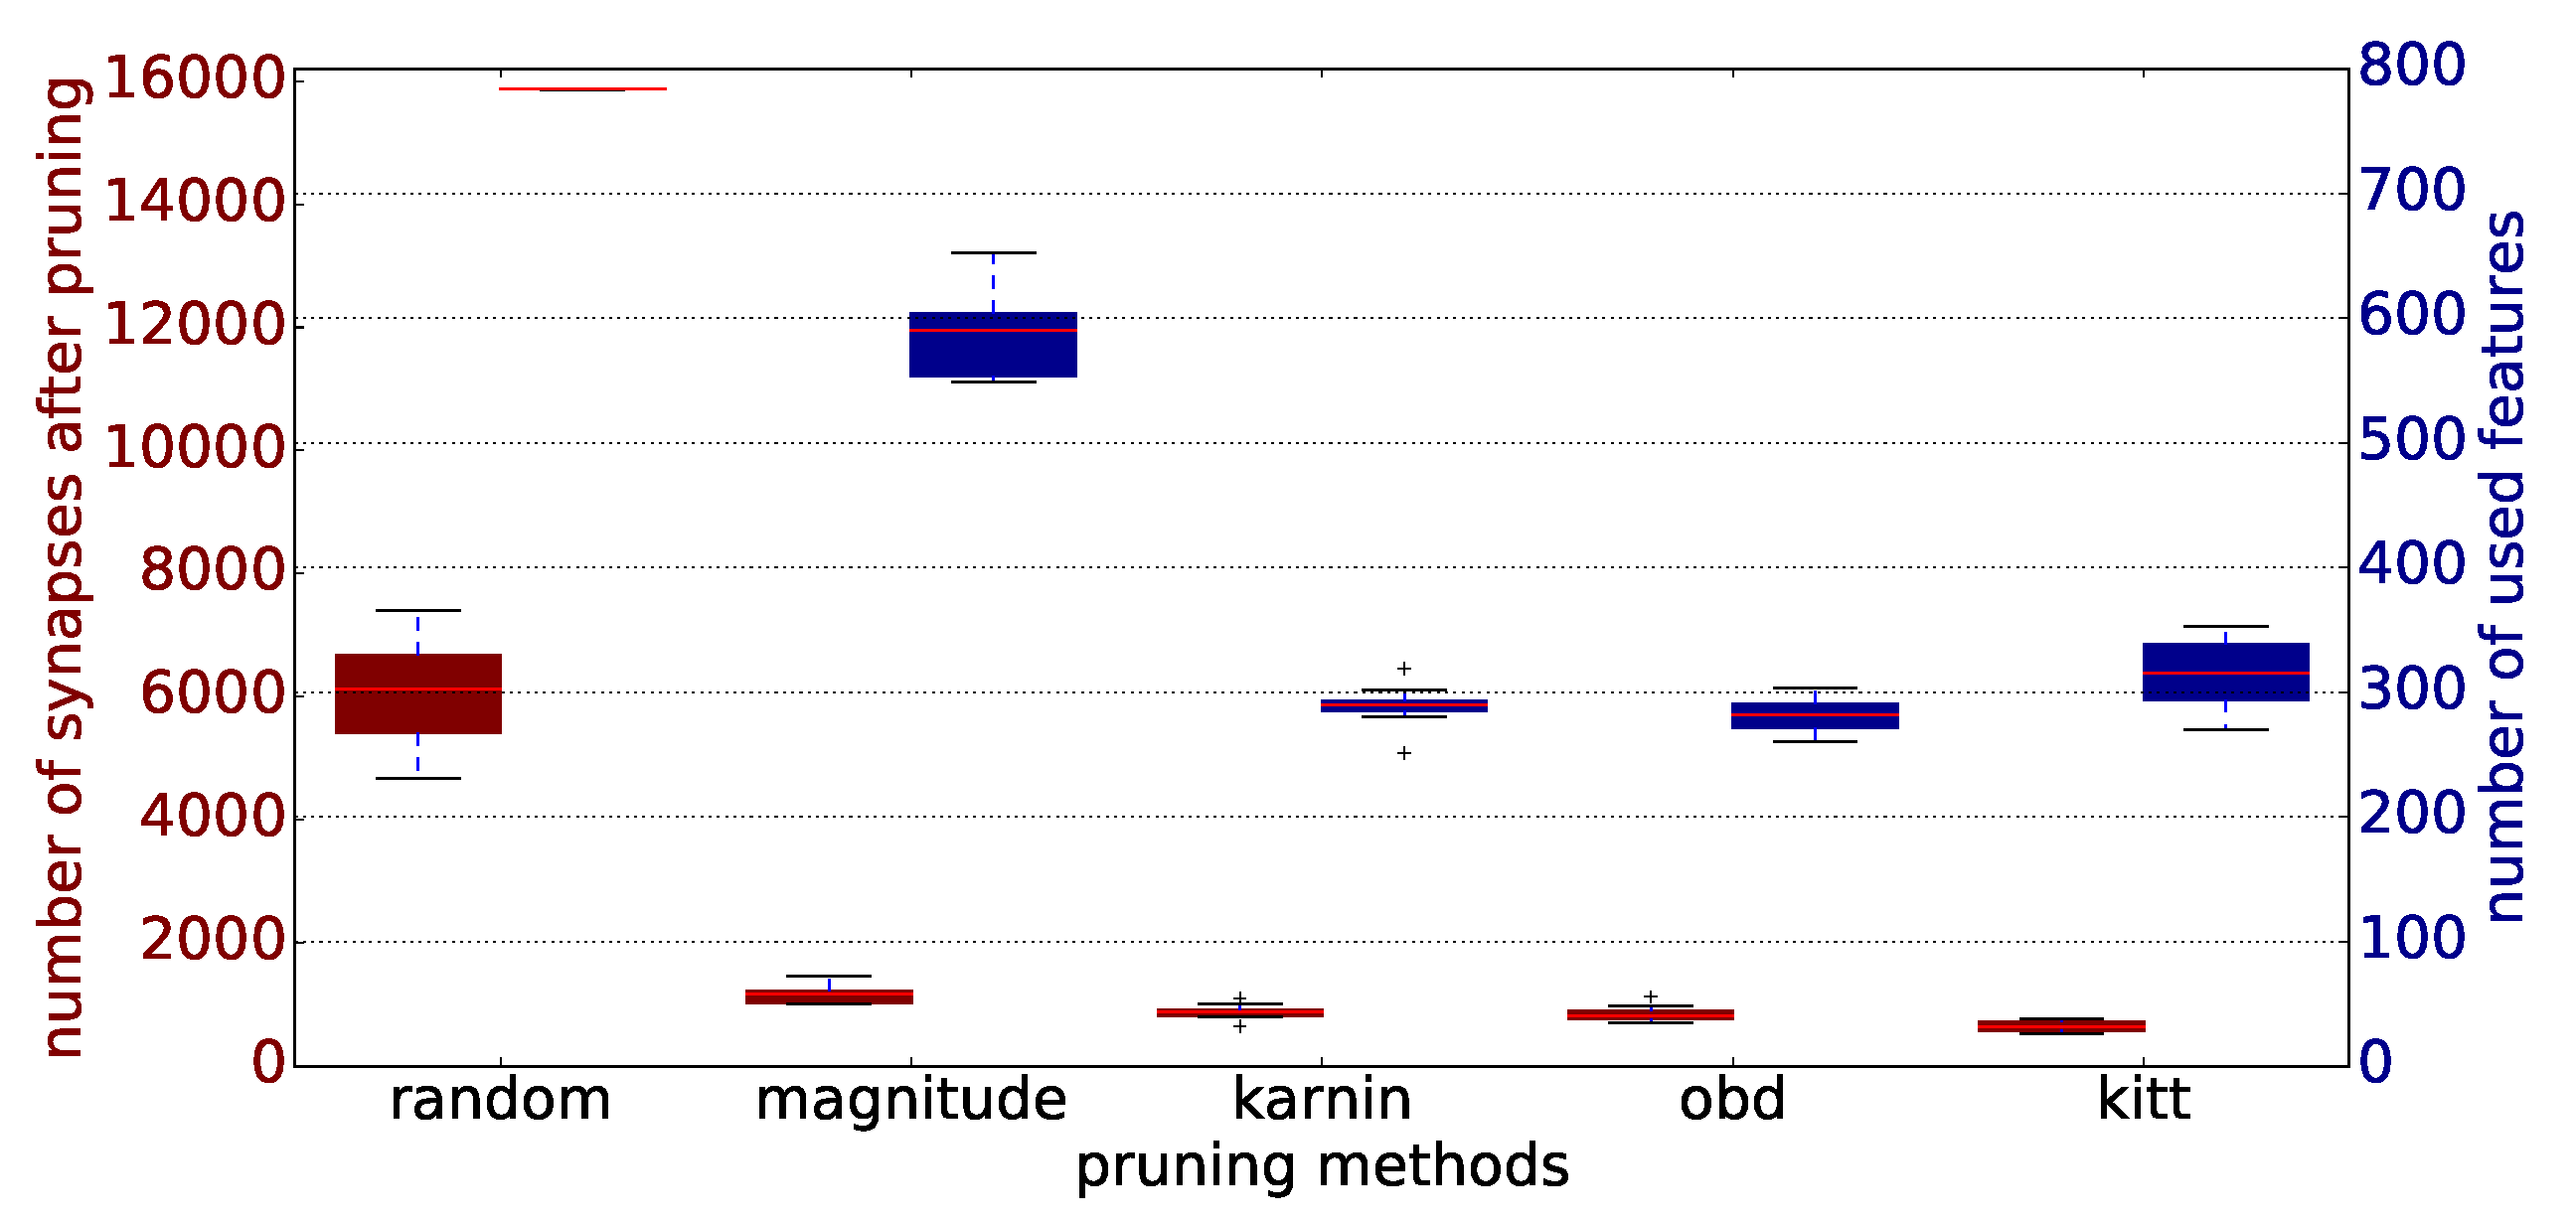
\includegraphics[width=\textwidth]{pa_comparison_retraining5.eps}
\caption{MNIST, req\_acc = 0.95, retraining: 5 epochs}
\label{fig:discussion:pa_comparison_retraining5}
\end{figure}

\newpage

\begin{figure}[H]
\centering
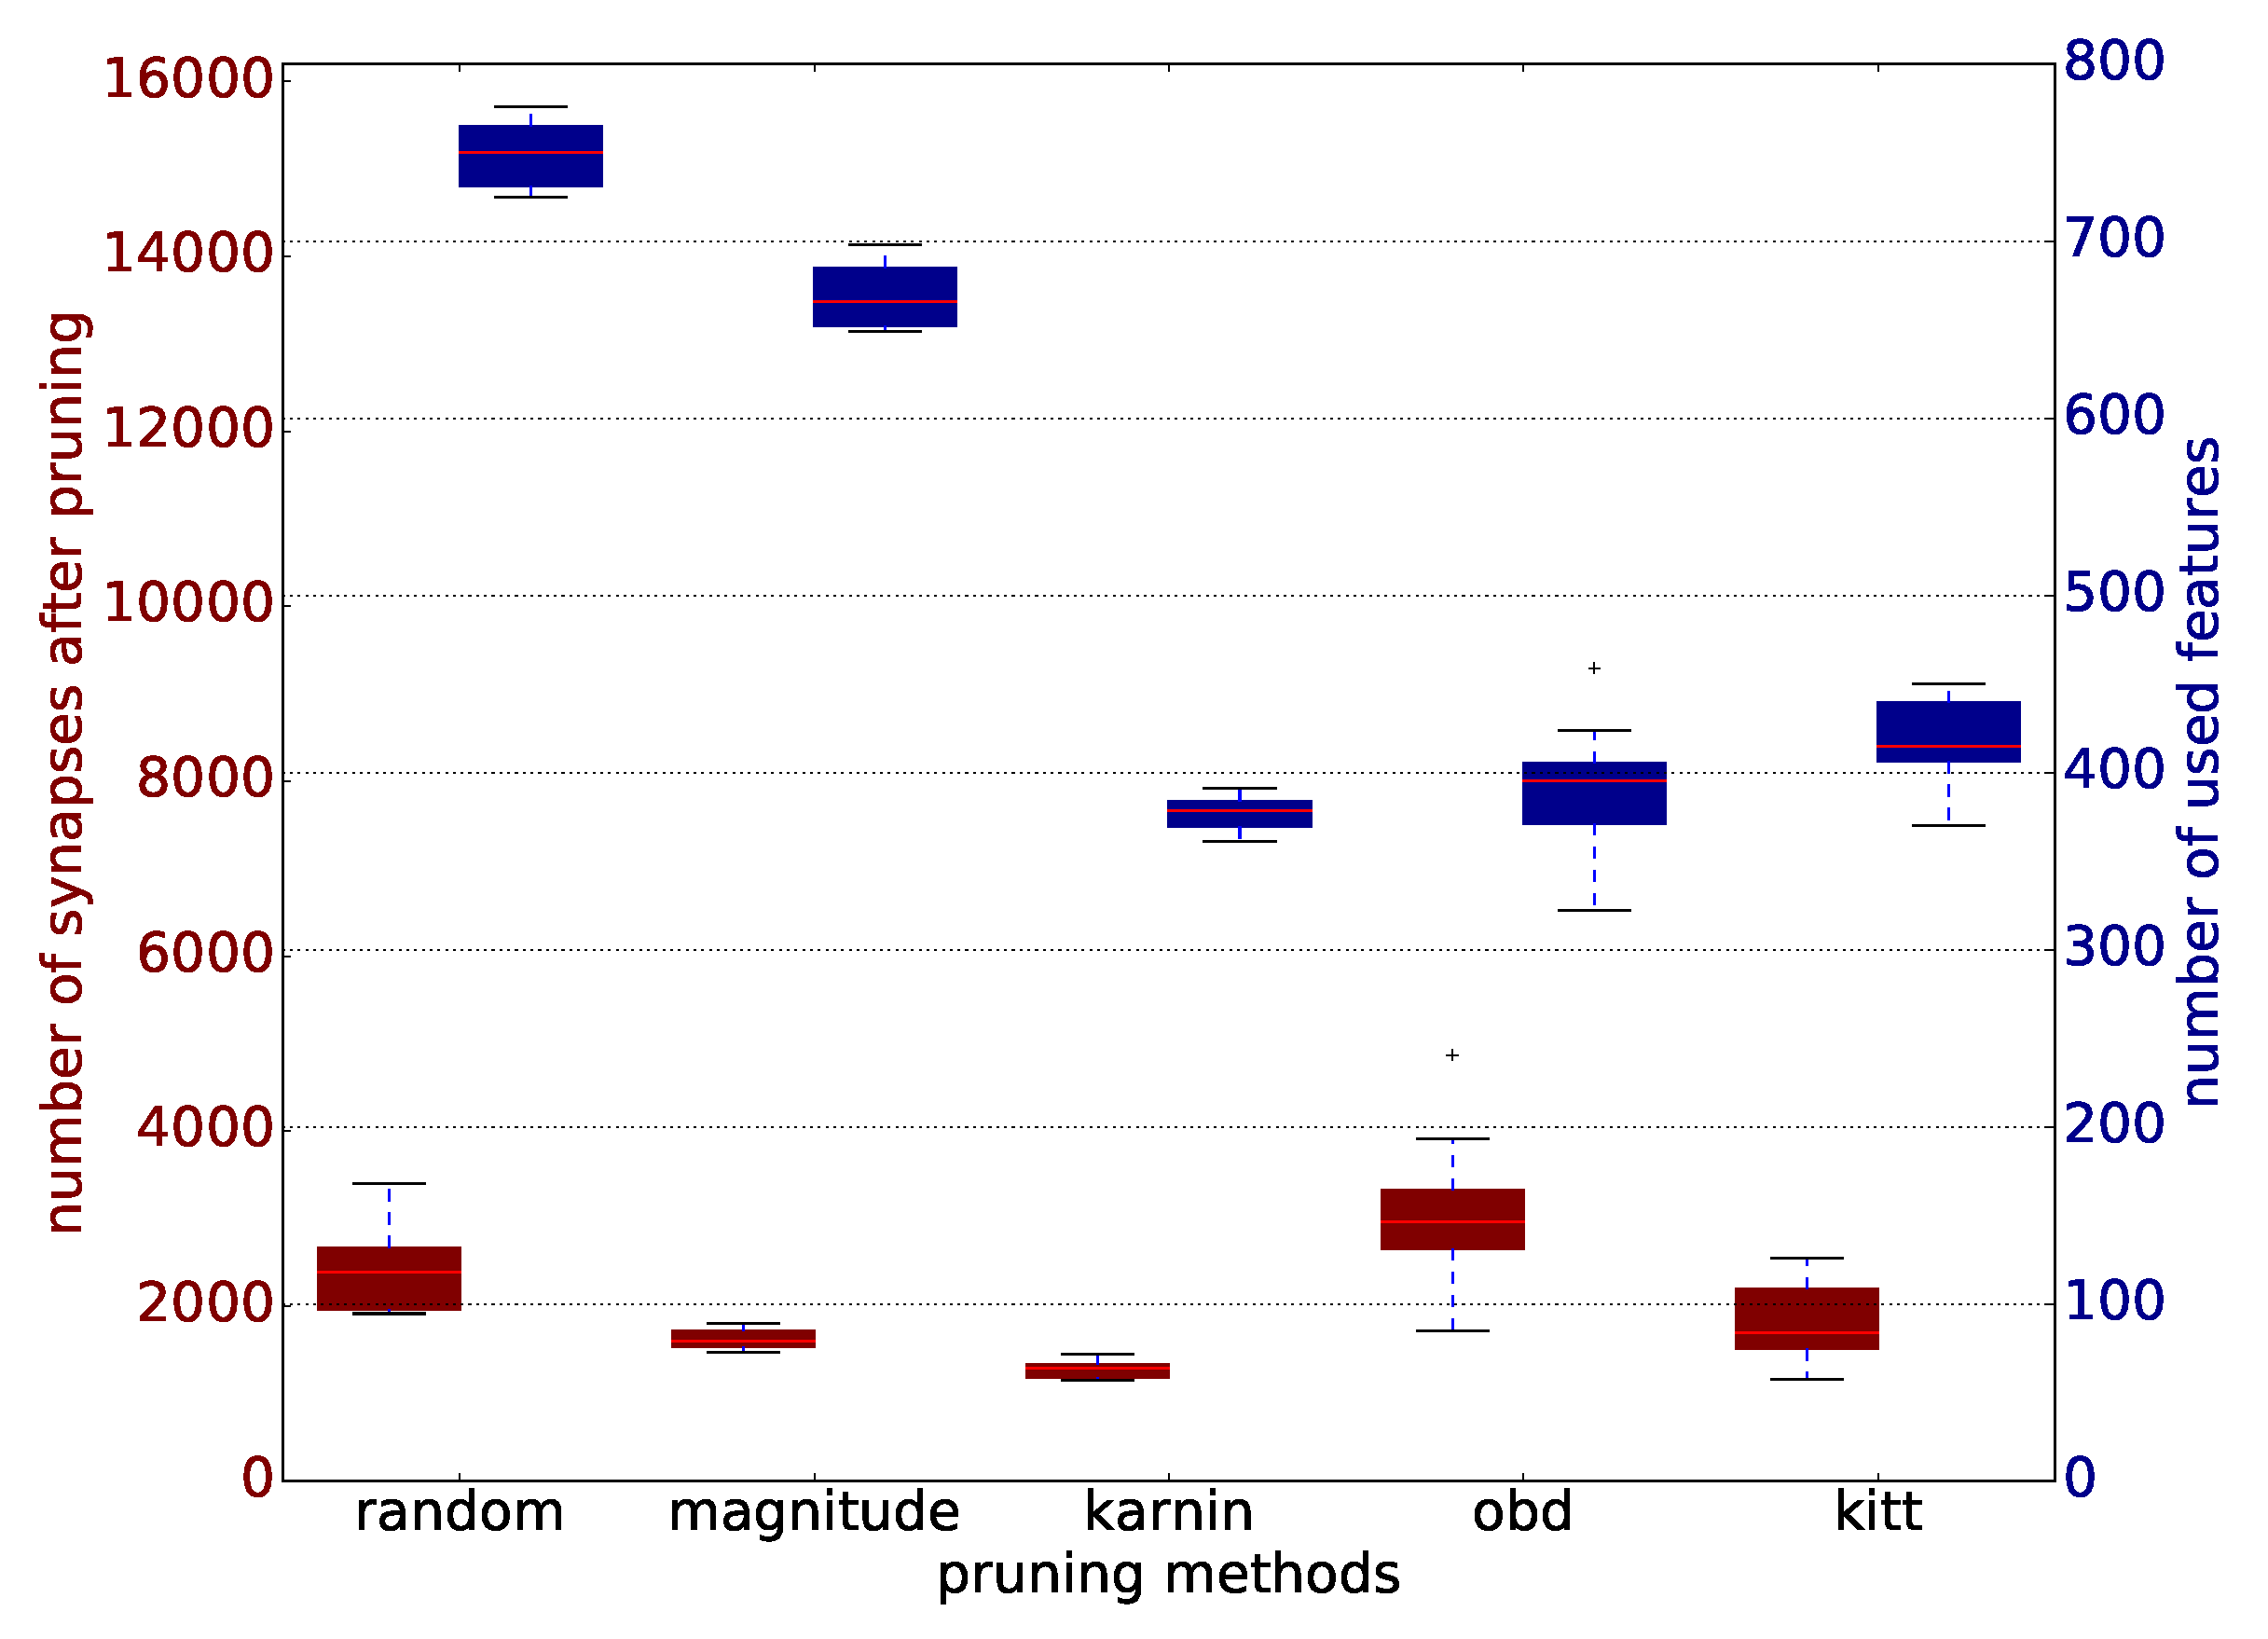
\includegraphics[width=\textwidth]{pa_comparison_noretraining.eps}
\caption{MNIST, req\_acc = 0.95, no retraining}
\label{fig:discussion:pa_comparison_noretraining}
\end{figure}

\section{Future Work} \label{sec:future_work}
Outlook...

Shrinking of layers

Tailoring

Building net from zero

Sphere neuron